%&../settings/preamble.main

\ifsubfile
\pagestyle{plain}
\setcounter{chapter}{4}

% NOTE sopprimere i warnings localmente
% \hbadness=10000
% \hfuzz=\maxdimen\newdimen\hfuzz
% % \usepackage[saveall]{silence}
% \usepackage{silence}
% \WarningsOff[caption]

% arara: pdflatex: { options: ["--output-directory=../build/chapters"], draft: yes, synctex: no }
% arara: pdflatex: { options: ["--output-directory=../build/chapters"], synctex: no }
\begin{document}
\fi
\chapter{Alberi}

% TODO scrivere introduzione

\section{Definizioni}

\begin{definition}[albero radicato, \foreign{rooted tree}]
Un albero consiste di un insieme di nodi e un insieme di archi orientati che connettono coppie di nodi, con le seguenti proprietà:
\begin{itemize}
	\item un nodo dell'albero è designato come nodo radice;
	\item ogni nodo \(n\), a parte la radice, ha esattamente un arco entrante;
	\item esiste un cammino unico dalla radice ad ogni nodo;
	\item l'albero è connesso.
\end{itemize}
\end{definition}

\begin{definition}[albero radicato, definizione ricorsiva]
Un albero è dato da:
\begin{itemize}
	\item un insieme vuoto, oppure
	\item una radice e zero o più sottoalberi, ognuno dei quali è albero; la radice è connessa alla radice di ogni sottoalbero con un arco orientato.
\end{itemize}
\end{definition}

\begin{definition}[profondità, \foreign{depth}]
La lunghezza del cammino semplice dalla radice al nodo (misurato in archi).
\end{definition}

\begin{definition}[livello, \foreign{level}]
L'insieme dei nodi alla stessa profondità.
\end{definition}

\begin{definition}[altezza dell'albero, \foreign{height}]
La profondità massima delle sue foglie.
\end{definition}

\section{Terminologia}

\begin{minipage}[c]{.45\textwidth}
	\centering
	\begin{itemize}[itemsep=5pt]
		\item \(A\) è la radice (\foreign{root});
		\item \(B\), \(C\) sono radici dei sottoalberi (\foreign{roots of their subtrees});
		\item \(D\), \(E\) sono fratelli (\foreign{siblings});
		\item \(D\), \(E\) sono figli (\foreign{children}) di \(B\);
		\item \(B\) è il padre (\foreign{parent}) di \(D\), \(E\);
		\item \(H\), \(I\), \(J\), \(K\), \(L\), \(M\), \(G\) sono foglie (\foreign{leafs});
		\item gli altri nodi sono nodi interni (\foreign{internal nodes});
		\item \(E\) è lo zio (il fratello del padre) di \(I\);
		\item \(B\) è il nonno di \(I\), \(I\) è il nipote di \(B\).
		% \item \(A\) è il bis-nonno di \(I\).
	\end{itemize}
\end{minipage}%
\begin{minipage}[c]{.45\textwidth}
	\centering
	\scalebox{.9}{
		\begin{forest} circled, wide
			[A [B [D [H][I]] [E [J][K]] ] [C [F [L][M]] [G] ]]
		\end{forest}
	}
\end{minipage}

\clearpage
\section{Alberi binari}

\begin{definition}[Albero binario]
Un albero binario è un albero radicato in cui ogni nodo ha al massimo due figli, che vengono identificati come figlio sinistro e figlio destro.
\end{definition}

\begin{note}
Due alberi \(T\) e \(U\) che hanno gli stessi nodi, gli stessi figli per ogni nodo e la stessa radice, sono distinti qualora un nodo \(u\) sia designato come figlio sinistro di un nodo \(v\) in \(T\) come figlio destro del medesimo nodo in \(U\).
In altre parole, anche se due alberi hanno lo stesso numero di nodi ed ognuno di questi nodi ha lo stesso numero di figli non è che detto che l'albero risultante sia identico.
\end{note}

\begin{algorithm}[H]
\caption*{Specifica albero binario}
%&../preamble

% arara: pdflatex: { synctex: no }
% arara: latexmk: { clean: partial }
\ifstandalone
\begin{document}
\begin{algorithm}[H]
\fi

\BlankLine
\tcp{GESTIONE ALBERO}

\BlankLine
\treeConstructor{\Item \(v\)} \Comment*[l]{costruisce un nuovo nodo, contenente \(v\), senza figli o genitori}
\Item \treeRead \Comment*[l]{legge il valore memorizzato nel nodo}
\treeWrite{\Item \(v\)} \Comment*[l]{modifica il valore memorizzato nel nodo}
\Tree \treeParent \Comment*[l]{restituisce il padre, oppure \Nil se questo nodo è radice}

\BlankLine
\BlankLine
\tcp{GESTIONE STRUTTURA}

\BlankLine
\tcp{restituiscono il figlio sinistro (destro) di questo nodo,}
\tcp{restituisce \Nil se assente}
\Tree \treeLeft\;
\Tree \treeRight\;

\BlankLine
\tcp{inserisce il sottoalbero radicato in \(t\)}
\tcp{come figlio sinistro (destro) di questo nodo}
\insertLeft{\Tree \(t\)}\;
\insertRight{\Tree \(t\)}\;

\BlankLine
\tcp{distrugge (ricorsivamente) il figlio sinistro (destro) di questo nodo}
\deleteLeft\;
\deleteRight\;

\ifstandalone
\end{algorithm}
\end{document}
\fi

\end{algorithm}

\begin{note}
Le funzioni \emph{senza parametri} sono indicate con un carattere senza grazie e privi di parentesi tonde vuote al fine di alleggerire la lettura del codice.
\end{note}

\subsection{Memorizzazione di un albero binario}

\begin{figure}[H]
	\centering
	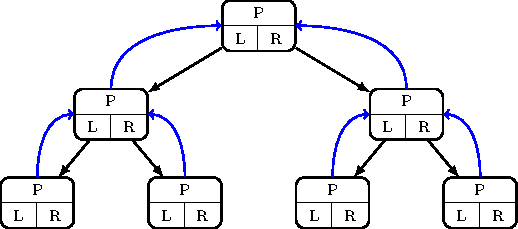
\includegraphics{tree-binary}
\end{figure}

Vengono memorizzati i seguenti campi:
\begin{itemize}
	\item \emph{parent}: riferimento al nodo padre;
	\item \emph{left}: riferimento al figlio sinistro;
	\item \emph{right}: riferimento al figlio destro.
\end{itemize}
Uno qualunque di questi oggetti potrebbe essere pari a \Nil, stando ad indicare che non esiste nessun sottoalbero.

\subsection{Implementazione}

\begin{algorithm}[H]
	\caption{Implementazione albero binario in pseudocodice}
	%&../preamble

% arara: pdflatex: { synctex: no }
% arara: latexmk: { clean: partial }
\ifstandalone
\begin{document}
\begin{algorithm}[H]
\fi
\begin{minipage}[t]{.5\textwidth}

\tcp{crea un nuovo albero}
\tcp{restituisce la radice dell'albero creato}
\prototype{\Tree \treeConstructor{\Item \(v\)}}{
	\Tree \(t =\) \new \Tree\;
	\(t.\varParent \Assign \Nil\)\;
	\(t.\varLeft \Assign t.\varRight \Assign \Nil\)\;
	\(t.\Value \Assign v\)\;

	\BlankLine
	\Return \(t\)\;
}

\prototype{\insertLeft{\Tree \(t\)}}{
	\If{\(\varLeft \Neq \Nil\)}{
		\(t.\varParent \Assign \This\)\;
		\(\varLeft \Assign t\)\;
	}
}

\prototype{\insertRight{\Tree \(t\)}}{
	\If{\(\varRight \Neq \Nil\)}{
		\(t.\varParent \Assign \This\)\;
		\(\varRight \Assign t\)\;
	}
}

\end{minipage}% <- importante, non toccare!
\begin{minipage}[t]{.5\textwidth}

\tcp{elimina ricorsivamente il sottoalbero sinistro}
\prototype{\deleteLeft{}}{
	\If{\(\varLeft \Neq \Nil\)}{
		\(\varLeft.\deleteLeft\)\;
		\(\varLeft.\deleteRight\)\;
		\(\varLeft \Assign \Nil\)\;
	}
}

\tcp{elimina ricorsivamente il sottoalbero destro}
\prototype{\deleteRight{}}{
	\If{\(\varRight \Neq \Nil\)}{
		\(\varRight.\deleteLeft\)\;
		\(\varRight.\deleteRight\)\;
		\(\varRight \Assign \Nil\)\;
	}
}

\end{minipage}
\ifstandalone
\end{algorithm}
\end{document}
\fi

\end{algorithm}

\subsection{Visite}

La visita di un albero (o la ricerca) è una strategia per passare attraverso (visitare) tutti i nodi di un albero.
Si possono distinguere due tipi di visite:
\begin{enumerate}
	\item visita in profondità: chiamata anche \foreign{Depth-First Search} (DFS), per visitare un albero visita ricorsivamente ognuno dei suoi sottoalberi; esistono tre varianti in base a quando il nodo viene visitato (pre, in o post-ordine); questa particolare visita sfrutta implicitamente il meccanismo di una pila (\foreign{stack}) tramite le chiamate ricorsive effettuate;
	\item visita in ampiezza: chiamata anche \foreign{Breadth First Search} (BFS), per visitare un albero visita ogni livello, uno dopo l'altro partendo dalla radice; richiede esplicitamente l'utilizzo di una coda (\foreign{queue}).
\end{enumerate}

\begin{algorithm}[H]
	\caption{Schema per visita in profondità}
	%&../preamble

% arara: pdflatex: { synctex: no }
% arara: latexmk: { clean: partial }
\ifstandalone
\begin{document}
\begin{algorithm}[H]
\fi
\begin{minipage}[t]{.5\linewidth}

\BlankLine
\prototype{\dfsSchema{\Tree \(t\)}}{
	\If{\(t \neq \Nil\)}{

		\BlankLine
		\tcp{pre-order visit}
		\Print \(t\)\;

		\BlankLine
		\dfsProc{\(t.\treeLeft\)}\;

		\BlankLine
		\tcp{in-order visit}
		\Print \(t\)\;

		\BlankLine
		\dfsProc{\(t.\treeRight\)}\;

		\BlankLine
		\tcp{post-order visit}
		\Print \(t\)\;
	}
}

\end{minipage}%
\begin{minipage}[t]{.5\linewidth}

\ifFigureOfAlgo
\begin{minipage}[t][5cm]{.5\linewidth}
	\centering
	\vfill
	\begin{forest} circled, for tree={font=\footnotesize\scshape}
		[a
			[b
				[c]
				[d]
			]
			[e
				[f]
				[g]
			]
		]
	\end{forest}
	\vfill
	\begin{tabular}{@{} l *{7}{ >{\scshape}c @{} } @{}}\small
		\emph{pre}-visita  & a & b & c & d & e & f & g \\
		\emph{in}-visita   & c & b & d & a & f & e & g \\
		\emph{post}-visita & c & d & b & f & g & e & a \\
	\end{tabular}
\end{minipage}
\fi

\end{minipage}
\ifstandalone
\end{algorithm}
\end{document}
\fi

\end{algorithm}

A seconda di dove scrivo il codice in questo schema ottengo una visita diversa.

\clearpage
\subsection{Applicazioni}

In genere post-visita e in-visita sono quelle più applicate, la pre-visita meno.

\subsection*{Visita in post-ordine}

Una possibile applicazione della visita post-ordine è quella di effettuare un conteggio dei nodi presenti nell'albero.

\begin{algorithm}[H]
	\caption{Conteggio dei nodi in un albero}
	%&../preamble

% arara: pdflatex: { synctex: no }
% arara: latexmk: { clean: partial }
\ifstandalone
\begin{document}
\begin{algorithm}[H]
\fi
\begin{minipage}[c]{.4\textwidth}

\prototype{\conteggioNodi{\Tree \(t\)}}{
	\eIf{\(t \Equal \Nil\)}{
		\tcp{è un albero vuoto}
		\Return \(0\)\;
	}{
		\tcp{conto ricorsivamente i nodi}
		\(C_{\ell} = \conteggioNodi{\(t.\treeLeft\)}\)\;
		\(C_{r} = \conteggioNodi{\(t.\treeRight\)}\)\;

		\BlankLine
		\Return \(C_{\ell} + C_{r} + 1\)\;
	}
}

\end{minipage}%
\begin{minipage}[c]{.5\textwidth}%
\ifFigureOfAlgo%
\hfill% centramento orizzontale
\begin{minipage}[t][3.8cm]{.85\linewidth}
	\centering
	\begin{forest} circled, wide,
		for tree={
			font=\scshape,
			count/.style 2 args={
				edge label={node[near end, font=\sffamily\scriptsize, #1]{#2}},
		    },
		}
		[a
			[b, count={above left}{3}
				[c, count={above left}{1}]
				[d, count={above right}{1}]
			]
			[e, count={above right}{3}
				[f, count={above left}{1}]
				[g, count={above right}{1}]
			]
		]
	\end{forest}
\end{minipage}
\fi
\end{minipage}
\ifstandalone
\end{algorithm}
\end{document}
\fi

\end{algorithm}

\subsection*{Visita in ordine (in-visita)}

Una possibile applicazione della visita post-ordine è quella di stampare espressioni con operatori binari.

\begin{algorithm}[H]
	\caption{Stampa espressioni con operatori binari}
	%&../preamble

% arara: pdflatex: { synctex: no }
% arara: latexmk: { clean: partial }
\ifstandalone
\begin{document}
\begin{algorithm}[H]
\fi
\begin{minipage}{.5\textwidth}

\prototype{\Int \stampaEspressioni{\Tree \(t\)}}{
	\eIf{\(t.\treeLeft \Equal \Nil\) \And \(t.\treeRight \Equal \Nil\)}{
		\tcp{siamo in una foglia}
		\Print \(t.\treeRead\)
	}{
		\tcp{sono su un nodo interno}
		\Print \enquote{(}\;

		\stampaEspressioni{\(t.\treeLeft\)}\;

		\Print \(t.\treeRead\)\;

		\stampaEspressioni{\(t.\treeRight\)}\;

		\Print \enquote{)}\;
	}
}

\end{minipage}%
\begin{minipage}{.5\textwidth}
\ifFigureOfAlgo
\begin{minipage}[t][4.5cm]{.85\linewidth}
	\vfill\centering
	\begin{center}
		\begin{forest} circled math tree
		[*[+[4][9]][+[3][4]]]
		\end{forest}
	\end{center}
	Stampa: \texttt{(( 4 + 9 ) * ( 3 + 4 ))}
	\vfill
\end{minipage}
\fi

\end{minipage}
\ifstandalone
\end{algorithm}
\end{document}
\fi

\end{algorithm}

% TODO
% Questa particolare funzione è stata utilizzata nell'esame del

\subsection*{Complessità di una visita}

Il costo di una visita di un albero contenente \(n\) nodi è \(\Theta(n)\), in quanto ogni nodo viene visitato al massimo una volta.

\clearpage
\section{Alberi generici}

\begin{algorithm}[H]
	\caption{Specifica albero generico}
	%&../preamble

% arara: pdflatex: { synctex: no }
% arara: latexmk: { clean: partial }
\ifstandalone
\begin{document}
\begin{algorithm}[H]
\fi

\BlankLine
\tcp{GESTIONE ALBERO}

\BlankLine
\treeConstructor{\Item \(v\)} \Comment*[l]{costruisce un nuovo nodo, contenente \(v\), senza figli o genitori}
\Item \treeRead \Comment*[l]{legge il valore memorizzato nel nodo}
\treeWrite{\Item \(v\)} \Comment*[l]{modifica il valore memorizzato nel nodo}
\Tree \treeParent \Comment*[l]{restituisce il padre, oppure \Nil se questo nodo è radice}

\BlankLine
\BlankLine
\tcp{GESTIONE STRUTTURA}

\begin{minipage}{\textwidth}%
\begin{multicols}{2}%

\BlankLine
\tcp{restituiscono il primo figlio,}
\tcp{oppure \Nil se questo nodo è una foglia}
\Tree \treeChild\;

\BlankLine
\tcp{restituisce il prossimo fratello,}
\tcp{oppure \Nil se assente}
\Tree \treeSibling\;

\BlankLine
\tcp{inserisce il sottoalbero \(t\)}
\tcp{come primo figlio di questo nodo}
\insertChild{\Tree \(t\)}

\BlankLine
\tcp{inserisce il sottoalbero \(t\)}
\tcp{come prossimo fratello di questo nodo}
\insertSibling{\Tree \(t\)}

\BlankLine
\tcp{distuggi l'albero radicato}
\tcp{identificato dal primo fratello}
\deleteChild

\BlankLine
\tcp{distuggi l'albero radicato}
\tcp{identificato dal primo figlio}
\deleteSibling

\end{multicols}
\end{minipage}
\vspace{5pt}

\ifstandalone
\end{algorithm}
\end{document}
\fi

\end{algorithm}

\subsection{Visita in profondità}

Un albero binario è anche un albero generale e lo visitiamo esattamente come lo visitavamo prima.

\begin{algorithm}[H]
	\caption{Visita in profondità}
	%&../preamble

% arara: pdflatex: { synctex: no }
% arara: latexmk: { clean: partial }
\ifstandalone
\begin{document}
\begin{algorithm}[H]
\fi

\BlankLine
\prototype{\dfsProc{\Tree \(t\)}}{
	\If{\(t \neq \Nil\)}{

		\BlankLine
		\tcp{pre-order visit}
		\Print \(t\)\;

		\BlankLine
		\dfsProc{\(t.\treeLeft{}\)}\;

		\BlankLine
		\tcp{effettuo visita}
		\Tree \(u\) \Assign \(t\).\treeChild\;
		\While{\(u \Neq \Nil\)}{
			\dfsProc{\(u\)}\;
			\(u\).\treeSibling\;
		}

		\BlankLine
		\tcp{post-order visit}
		\Print \(t\)\;
	}
}

\ifstandalone
\end{algorithm}
\end{document}
\fi

\end{algorithm}

\subsection{Visita in ampiezza}

Mentre nella visita in profondità il meccanismo della pila (\foreign{stack}) era implicito nelle chiamate ricorsive, in questo caso è necessario utilizzare \emph{esplicitamente} una coda (\foreign{queue}).
Un'altra differenza fra i due algoritmi è che quello in profondità è un algoritmo ricorsivo, l'altro è iterativo.
Quando tutti i nodi di un livello vengono estratti dalla coda, la coda contiene solo ed unicamente i nodi del livello successivo.

\begin{algorithm}[H]
	\caption{Visita in ampiezza}
	%&../preamble

% arara: pdflatex: { synctex: no }
% arara: latexmk: { clean: partial }
\ifstandalone
\begin{document}
\begin{algorithm}[H]
\fi
\begin{minipage}{.5\textwidth}

\prototype{\bfsProc{\Tree \(t\)}}{
	\Queue \(Q \Assign\) \queueConstructor\;
	\(Q.\queueInsert{t}\) \Comment*[l]{inserisci la radice}

	\BlankLine
	\While{\Not \(Q.\queueEmpty\)}{
		\tcp{fintanto che la coda non è vuota}
		\tcp{estraggo un nodo dalla coda}
		\Tree \(u \Assign Q.\queueRemove\)\;

		\BlankLine
		\tcp{visita per livelli del nodo \(u\)}
		\Print \(u\)\;

		\BlankLine
		\tcp{fintanto che ho almeno un figlio}
		\(u \Assign u.\treeChild\)\;
		\While{\(u \Neq \Nil\)}{

			\BlankLine
			\tcp{metto in coda il figlio}
			\(Q.\queueInsert{u}\)\;
			\tcp{passo al figlio destro}
			\(u \Assign u.\treeSibling\)\;
		}
	}
}

\end{minipage}%
\begin{minipage}{.5\textwidth}

\ifFigureOfAlgo
\begin{minipage}[t][7.5cm]{.85\linewidth}
	\vfill\centering
	\begin{center}
		\begin{forest} circled, wide
		[\textsc{a}[\textsc{b}[\textsc{c}][\textsc{d}]][\textsc{e}[\textsc{f}][\textsc{g}]]]
		\end{forest}
	\end{center}
	Sequenza: {\scshape a b e c d f g}
	\vfill\null
\end{minipage}
\fi

\end{minipage}
\ifstandalone
\end{algorithm}
\end{document}
\fi

\end{algorithm}

\paragraph{Commento}
Mettiamo in coda tutti i nodi che vogliamo visitare passo passo.
Qui la stampa è in pre-visita ma qui -- a differenza dei grafi -- non ha molta importanza se la visita la facciamo prima o dopo.
Visito tutti i figli prima di passare al livello successivo.

\section{Memorizzazione}

Esistono diversi modi per memorizzare un albero, più o meno indicati a seconda del numero massimo e medio di figli presenti.
Le realizzazioni possibili sono:
\begin{enumerate}
	\item con vettore dei figli;
	\item primo figlio, prossimo fratello;
	\item con vettore dei padri
\end{enumerate}

\subsection{Realizzazione con vettore dei figli}

\begin{figure}[H]
	\centering
	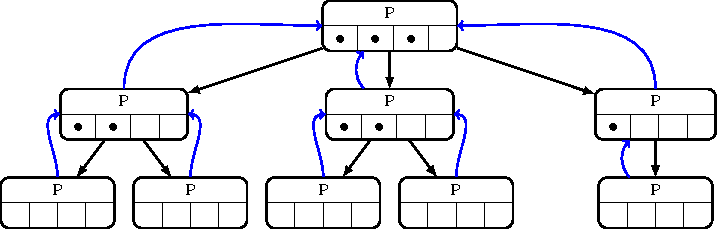
\includegraphics[width=.8\textwidth]{tree-vectorChildren}
	\caption[Realizzazione di un albero tramite vettore dei figli]{Realizzazione con vettore dei figli}
	\label{fig:tree-vector-children}
\end{figure}

Vengono memorizzati i seguenti campi:
\begin{itemize}
	\item \emph{parent} che è il riferimento al nodo padre;
	\item vettore dei figli il quale a seconda del numero dei figli può comportare una discreta quantità di spazio sprecato.
\end{itemize}

\subsection{Realizzazione basata su primo figlio, prossimo fratello}

Viene implementato come una lista di fratelli.

\begin{figure}[H]
	\centering
	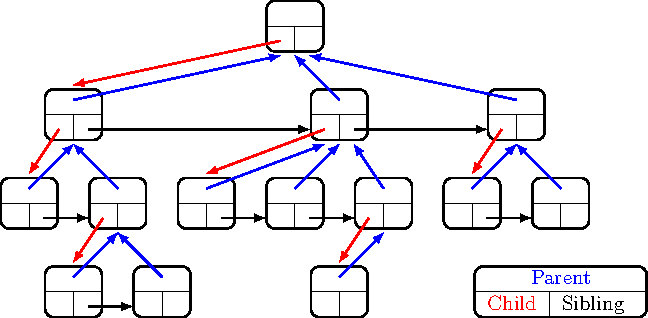
\includegraphics[width=.8\textwidth]{tree-listChildren}
	\caption[Realizzazione di un albero tramite primo figlio, prossimo fratello]{Realizzazione basata su primo figlio, prossimo fratello}
	\label{fig:tree-list-children}
\end{figure}

La memorizzazione che viene utilizzata nel \foreign{file system} è esattamente questa.

\begin{algorithm}[H]
	\caption{Implementazione albero \enquote{primo figlio, prossimo fratello} in pseudocodice}
	%&../preamble

% arara: pdflatex: { synctex: no }
% arara: latexmk: { clean: partial }
\ifstandalone
\begin{document}
\begin{algorithm}[H]
\fi

\Tree \varParent \Comment*[r]{Riferimento al padre}
\Tree \varChild \Comment*[r]{Riferimento al primo figlio}
\Tree \varSibling \Comment*[r]{Riferimento al prossimo fratello}
\Item \varValue \Comment*[r]{Valore memorizzato nel nodo}

\begin{minipage}{.5\textwidth}

\BlankLine
\prototype{\Tree \treeConstructor{\Item \(v\)}}{
	\Tree \(t =\) \new \Tree\;
	\(t.\varValue \Assign v\)\;
	\(t.\varParent \Assign t.\varChild \Assign t.\varSibling \Assign \Nil\)\;

	\BlankLine
	\Return \(t\)\;
}

\BlankLine
\prototype{\insertChild{\Tree \(t\)}}{
	\(t.\varParent \Assign \Self\)\;
	\tcp{inserisci \(t\) prima dell'attuale primo figlio}
	\(t.\varSibling \Assign \varChild\)\;
	\(\varChild \Assign t\)\;
}

\BlankLine
\prototype{\insertSibling{\Tree \(t\)}}{
	\(t.\varParent \Assign \varParent\)\;
	\tcp{inserisci \(t\) prima dell'attuale prossimo fratello}
	\(t.\varSibling \Assign \varSibling\)\;
	\(\varSibling \Assign t\)\;
}

\end{minipage}%
\begin{minipage}{.5\textwidth}

\BlankLine
\prototype{\deleteChild{}}{
	\(\Tree\ newChild\ \Assign \varChild.\treeSibling\)\;
	\delete{\varChild}\;
	\(\varChild \Assign newChild\)\;
}

\BlankLine
\prototype{\deleteSibling{}}{
	\(\Tree\ newBrother\ \Assign \varSibling.\treeSibling\)\;
	\treeDelete{\varSibling}\;
	\(\varSibling \Assign newBrother\)\;
}

\BlankLine
\tcp{metodo ausiliare}
\prototype{\treeDelete{\Tree \(t\)}}{
	\Tree \(u\) \Assign \(t\).\treeChild\;

	\BlankLine
	\While{\(u \Neq \Nil\)}{
		\Tree \(next\) \Assign \(u\).\treeSibling\;
		\treeDelete{\(u\)}\;
		\(u \Assign next\)\;
	}
}

\end{minipage}

\ifstandalone
\end{algorithm}
\end{document}
\fi

\end{algorithm}

\newpage
\subsection{Realizzazione con vettore dei padri}

Nella realizzazione con vettore dei padri, l'albero è rappresentato da un vettore i cui elementi contengono il valore associato al nodo e l'indice della posizione del padre del vettore.

\bigskip
\begin{minipage}[c]{.5\textwidth}
	\centering
	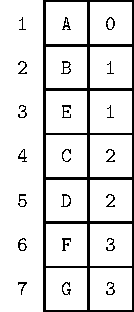
\includegraphics{tree-vectorParents}
\end{minipage}%
\begin{minipage}[c]{.5\textwidth}
	\centering
	\begin{forest} circled, wide, for tree={font=\scshape}
	[a[b[c][d]][e[f][g]]]
	\end{forest}
\end{minipage}

\bigskip
Questa realizzazione può sembrare particolarmente assurda poiché dato un nodo non permette di stabilire direttamente quali sono i suoi figli, ma ci sono molti algoritmi che sono interessati solo ai padri.
Questa è la rappresentazione più compatta che possiamo creare, vedremo la sua utilità quando andremo a studiare le visite sui grafi.

\ifsubfile
\end{document}
\fi
